% Created 2021-01-24 Sun 22:50
% Intended LaTeX compiler: pdflatex
\documentclass[11pt]{article}
\usepackage[utf8]{inputenc}
\usepackage[T1]{fontenc}
\usepackage{graphicx}
\usepackage{grffile}
\usepackage{longtable}
\usepackage{wrapfig}
\usepackage{rotating}
\usepackage[normalem]{ulem}
\usepackage{amsmath}
\usepackage{textcomp}
\usepackage{amssymb}
\usepackage{capt-of}
\usepackage{hyperref}
\usepackage{minted}
\hypersetup{colorlinks=true, linkcolor=black, filecolor=red, urlcolor=blue}
\usepackage[turkish]{babel}
\author{Eren Hatırnaz}
\date{25 Ağustos 2019}
\title{Yazılım Gündemi - 6\\\medskip
\large 12-25 Ağustos 2019}
\hypersetup{
 pdfauthor={Eren Hatırnaz},
 pdftitle={Yazılım Gündemi - 6},
 pdfkeywords={},
 pdfsubject={},
 pdfcreator={Emacs 27.1 (Org mode 9.3)},
 pdflang={Turkish}}
\begin{document}

\maketitle
\tableofcontents \clearpage\shorthandoff{=}

\begin{center}
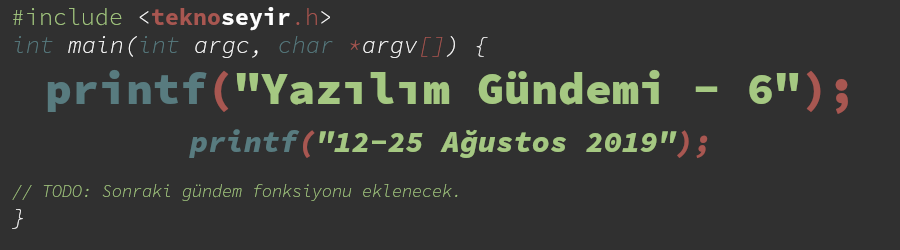
\includegraphics[width=.9\linewidth]{gorseller/yazilim-gundemi-banner.png}
\end{center}
\begin{center}
\href{../05/yazilim-gundemi-05.pdf}{< Önceki Gündem} | \textbf{12-25 Ağustos 2019} | \href{../07/yazilim-gundemi-07.pdf}{Sonraki Gündem >}

\href{https://teknoseyir.com/blog/yazilim-gundemi-6-12-25-agustos-2019}{TeknoSeyir'de Oku}
\end{center}

\section{RestClient ve diğer 10 Ruby kütüphanesinin \href{https://www.zdnet.com/article/backdoor-code-found-in-11-ruby-libraries/}{arka kapı içerdiği ortaya çıktı}}
\label{sec:org7fddd85}
Ruby kütüphanelerinin barındırıldığı \href{https://rubygems.org}{RubyGems.org} sitesindeki bilgileri çalınan
geliştiricilerin projelerine, kurulduğu sunucuda arka kapı açan kod parçaları
eklenmiş. Aynı olay strong-password isimli kütüphanenin de başına gelmişti
(bkz: \href{../01/yazilim-gundemi-01.pdf}{Yazılım Gündemi - 1}). Yöntem aynı: RubyGems.org sitesindeki kullanıcı
bilgilerini ele geçen hacker(lar), projeye zararlı kod parçaları eklemişler ve
yeni versiyon çıkarak, kütüphaneyi kullananların zararlı kod parçalarını
güncelleme ile edinmeleri sağlanmış.

\begin{figure}[htbp]
\centering
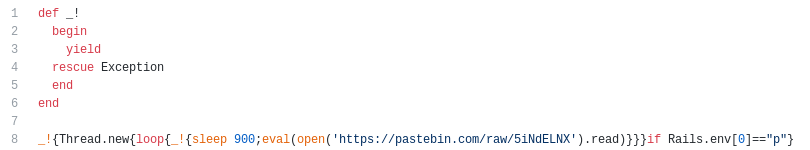
\includegraphics[width=.9\linewidth]{gorseller/ruby-zararli-kod.png}
\caption{CVE Numarası: \href{https://nvd.nist.gov/vuln/detail/CVE-2019-15224}{CVE-2019-15224}}
\end{figure}

Zararlı kod parçalarından bazıları kullanıcıların cookie bilgilerini çalmaya
yönelikken, bazıları da sistemi kripto para madenciliği için kullanıyormuş.
Daha teknik bilgiler için RestClient kütüphanesinin \href{https://github.com/rest-client/rest-client/issues/713}{şu github sayfası}na
bakabilirsiniz. Saldırıdan etkilenen Ruby kütüphaneleri ve versiyonları ise şu
şekilde:

\begin{itemize}
\item \textbf{rest-client}: \emph{1.6.10}, \emph{1.6.11}, \emph{1.6.12}, \emph{1.6.13}
\item \textbf{cron\_parser}: \emph{0.1.4}, \emph{1.0.12}, \emph{1.0.13}
\item \textbf{coin\_base}: \emph{4.2.1}, \emph{4.2.2}
\item \textbf{blockchain\_wallet}: \emph{0.0.6}, \emph{0.0.7}
\item \textbf{bitcoin\_vanity}: \emph{4.3.3}
\item \textbf{lita\_coin}: \emph{0.0.3}
\item \textbf{coming-soon}: \emph{0.2.8}
\item \textbf{omniauth\_amazon}: \emph{1.0.1}
\item \textbf{awesome-bot}: \emph{1.18.0}
\item \textbf{doge-coin}: \emph{1.0.2}
\item \textbf{capistrano-colors}: \emph{0.5.5}
\end{itemize}

Zararlı kod içerdikleri anlaşılan bu versiyonlar RubyGems.org ekibi tarafından
geri çekilmiş fakat olay anlaşına kadar bu kütüphaneler toplam 3.584 kez
indirilmiş. Siz de mutlaka projelerinizde yukarıdaki kütüphanelerin ve
versiyonların olup olmadığını kontrol edin ve tabii ki projenize bağımlılık
eklerken daha dikkatli olun.

\section{\texttt{standard} isimli JavaScript aracı terminal çıktısında \href{https://github.com/standard/standard/issues/1381}{reklam göstermeyi planlıyor}}
\label{sec:org14364d6}
GitHub'da 21K yıldıza sahip, başka bir çok proje tarafından da kullanılan bu
araç, fonlama konusunda yaşadığı sıkıntılardan ötürü terminal çıktısına açık
kaynağı destekleyen bir firmadan reklam almayı planlıyor. Yani projenize
\texttt{standard} aracını eklemek için \texttt{npm install standard} yazdığınızda aracın
kurulumu sonrasında terminalde ve muhtemelen log dosyasında bir reklam
göreceğiz. Açıkcası ben de şaşırdım fakat projenin github sayfasındaki issue
altında yazılanları görünce biraz da olsa hak verdim.

\begin{center}
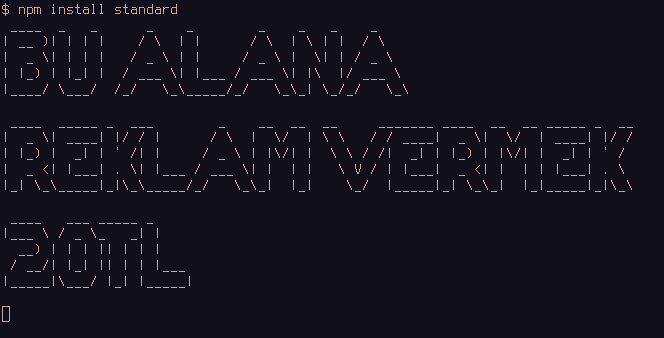
\includegraphics[width=.9\linewidth]{gorseller/terminal-reklam.png}
\end{center}

Hepimiz açık kaynağın nimetlerinden fazlasıyla faydalanıyoruz fakat açık
kaynak camiasına katkı sağlama konusunda ciddi eksikliklerimiz var. Girdiğimiz
açık kaynak projelerin sitelerindeki "Bağış Yap" butonlarını görmezden
geliyor, hatta sitedeki reklamları bile engelliyoruz. Üstüne bir de
karşılaştığımız sorunları ya da hataları çözmek için az da olsa uğraşmak
yerine direkt issue açıp ya da mail gönderip, 3-4 gün içerisinde sorumuzun
çözülmesini bekliyoruz. Lafa gelince hepimiz ortamlarda açık kaynağın
faydalarından, nimetlerinden, ne kadar süper bir şey olduğundan bahsettik;
fakat, konu maddi ve/veya manevi destek olmaya gelince ne elimizi cebimize
attık, ne de klavyemize dokunduk.

Terminal çıktısına reklam almak belki de doğru bir yöntem değil, fakat, şu çok
açık ortada ki: Geliştirici camiası olarak açık kaynak ile ilgili algılarımızı
değiştirme zamanımız geldi. Açık kaynak camiasından aldığımızın ne kadarını
geri verdiğimizin/verebildiğimizin sorusunu kendimize sormamız gerekiyor. Açık
kaynak araçları/kütüphaneleri kullanarak projeler yapıp bir güzel paramızı
kazanıyoruz ama hiç birimiz, "kardeşim ben senin projeni kullanarak para
kazandım, al bu da benden sana bu aracı geliştirmeye devam edebilmen için xx
\$/€" ya da "\#504 numaralı issue sayfasındaki sorunu çözdüm, inceleyip,
kodlarımı kabul edebilir misin?" demiyoruz. Ohh, ne rahat!\ldots{}

Bu konuda siz ne düşünüyorsunuz? Kullandığınız bir araç/kütüphane bu şekilde
reklam alsa -ki şu an almayı planlıyor- tepkiniz ne olurdu? Yorum kısmında
konuşalım.
\section{Git versiyon kontrol sisteminin \href{https://raw.githubusercontent.com/git/git/master/Documentation/RelNotes/2.23.0.txt}{2.23 sürümü duyuruldu}}
\label{sec:org49790e3}
Hepimizin her gün kullandığı popüler versiyon kontrol sistemi git 2.23 sürümü
ile yenilikler ve hata gidermelerini sunuyor. Öne çıkan bazı özellikler bu
şekilde:

\subsection{\texttt{git checkout} için yeni deneysel alternatif komutlar}
\label{sec:org27900a9}
Bildiğimiz gibi \texttt{git checkout} komutu hem dallar arasında geçiş yapmak için
hem de dosyaları son commit'deki hallerine resetlemek için kullanılabiliyor.
Üstelik \texttt{git checkout -{}-branch olmayan-dal} gibi bir kullanımla da olmayan
bir dalı yaratıp, ona geçiş yapma özelliği de var. İki farklı işlevin bir
komuta toplanmasından dolayı benim de zaman zaman garipsediğim bir komut. Bu
sürümde bu işlevleri ayıran deneysel iki komut eklenmiş.

\begin{itemize}
\item \textbf{\texttt{git switch}}: Dallar arasında geçiş yapmak, yeni dal oluşturup ona geçmek
için kullanılacak. \href{https://git-scm.com/docs/git-switch/2.23.0}{Dokümantasyon}. Örnek:
\begin{verbatim}
$ git switch yeni-ozellik

Switched to branch 'yeni-ozellik'
Your branch is up to date with 'origin/yeni-ozellik'
\end{verbatim}
\item \textbf{\texttt{git restore}}: Verilen dosyası son commit'deki haline geri döndürmek için
kullanılacak. \href{https://git-scm.com/docs/git-restore/2.23.0}{Dokümantasyon}. Örnek:
\begin{verbatim}
$ git restore program.c
\end{verbatim}
\end{itemize}

Diğer özellikler ve değişiklikler için konu başlığındaki bağlantıya
tıklayabilir ya da GitHub Blog'da yayınlanan \href{https://github.blog/2019-08-16-highlights-from-git-2-23/}{bu yazıyı} okuyabilirsiniz.
\section{Bitbucket, \href{https://bitbucket.org/blog/sunsetting-mercurial-support-in-bitbucket}{Mercurial desteğini sonlandırmaya} hazırlanıyor}
\label{sec:orgebb1745}
Bitbucket, GitHub gibi bir uzak depo sunucu hizmeti veren bir site. GitHub'dan
farklı olarak sadece git ile değil, alternatif bir versiyon kontrol sistemi
olan mercurial ile de çalışmayı destekliyordu. Fakat artık Bitbucket'da bu
desteğini sonlandırmaya karar vermiş ve planlar yapılmış. \emph{1 Şubat 2020}
itibariyle kullanıcılar \textbf{yeni Mercurial deposu} oluşturulamayacak; \emph{1 Haziran
2020} itibariyle de Bitbucket'de \textbf{Mercurial desteği tamamen kalkacak ve
Mercurial depoları da sunucudan silinecek}. Desteğin kalkmasının nedenini
söylemeye gerek yok sanırım. Artık hepimiz her yeni projede varsayılan olarak
git kullanmaya başladık. Açıkcası ben Mercurial hiç kullanmadım, hatta öyle
bir depo da hiç görmedim, bu yüzden nasıl bir sistem olduğu konusunda pek
fikrim yok.

Bu haberi duyan, \%100 açık kaynak ve özgür yazılım olarak geliştirilen
Sourcehut da bir blog yazısı yayınlayarak, Bitbucket'dan Mercurial
kullanıcılarını \href{https://sourcehut.org/blog/2019-08-21-sourcehut-welcomes-bitbucket-refugees/}{kendi sitesine davet etti}.
\section{\href{https://blog.qt.io/blog/2019/08/21/announcing-qt-mcus/}{Mikrokontrolcüler için Qt} kütüphanesi tanıtıldı}
\label{sec:orgec4859a}
\href{https://www.youtube.com/watch?v=p9\_Qy3kw1wc}{YouTube videosu} |	\href{https://www.qt.io/qt-for-mcu}{Ürün tanıtım sayfası}

C++ deneyimim konsola "Merhaba dünya" yazdırmaktan öteye gitmediği halde bu
gelişme beni bile heyecanlandırdı. Özellikle videodaki gibi düşük sistem
gereksinimleri ile çalışan cihazlarda akıcı ve güzel tasarımlı ekranlar
hazırlayabileceksek, mutlaka bir ara Qt kütüphanesini incelemem gerekecek.

Teknik detayları henüz açık değil fakat konuyla ilgili Qt takımı, 4 Eylül
tarihinde internet üzerinden soru\&cevap kısmının da olacağı bir webiner
düzenleyecek. Sanırım webiner boyunca çok daha teknik kavramları
anlatacaklardır. \href{https://www.qt.io/qt-for-mcu\#MCUWebinar}{Buradan} kendinize uygun saatteki webinere kayıt
olabilirsiniz.
\section{Etkinlik Duyurusu: \href{https://kommunity.com/istanbulphp/events/typed-properties-ve-dahasi-ile-php-74}{Typed Properties ve dahası ile PHP 7.4}}
\label{sec:org0ed109b}
\begin{center}
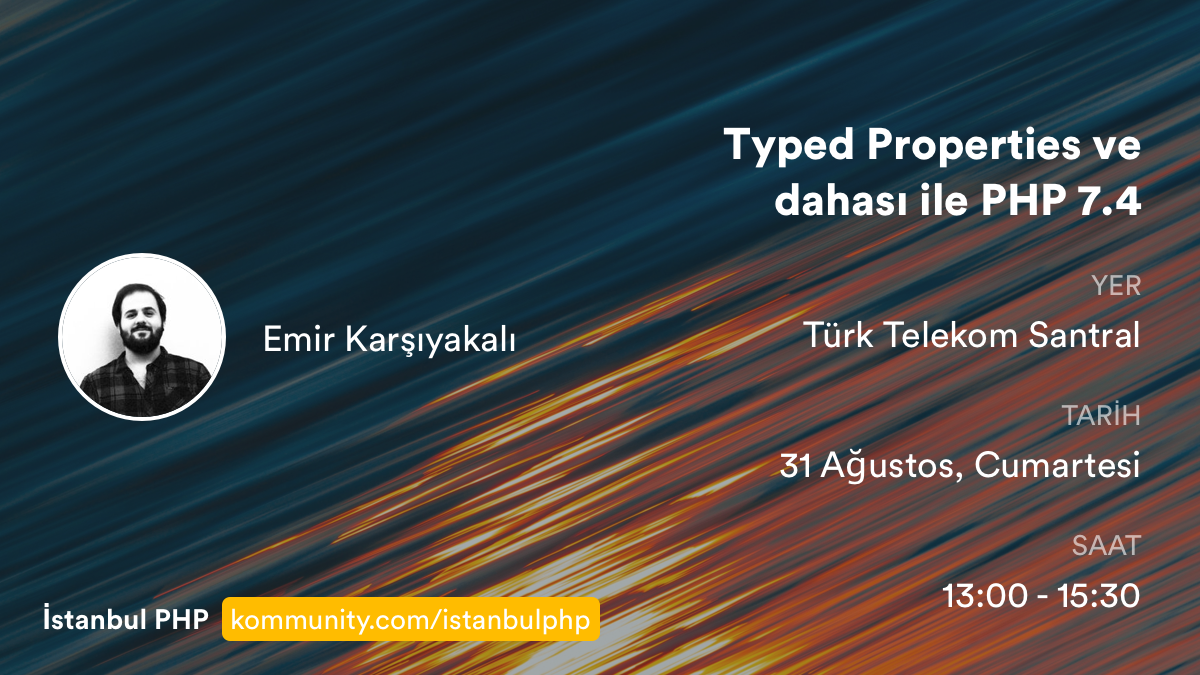
\includegraphics[width=.9\linewidth]{gorseller/php-etkinligi.png}
\end{center}

\href{https://twitter.com/istanbulphp}{İstanbul PHP grubu}nun organize ettiği bu etkinlikte PHP 7.4 ile birlikte
gelecek özellikler anlatılacak. Birkaç özelliği \href{../03/yazilim-gundemi-03.pdf}{Yazılım Gündemi - 3} yazısında
ben de anlatmıştım fakat PHP geliştirmeyle ilgilenen ve İstanbul'da olan
arkadaşların mutlaka bu etkinliğe katılmasını tavsiye ederim, daha faydalı
olacaktır.
\section{Diğer Haberler}
\label{sec:orgb21bb45}
\begin{itemize}
\item Netflix güvenlik takımı, \href{https://github.com/Netflix/security-bulletins/blob/master/advisories/third-party/2019-002.md}{HTTP/2 protokolünün de DoS saldırına karşı açık
olduğu}nu ortaya çıkardı.
\item \href{https://webkit.org/tracking-prevention-policy/}{WebKit Takip Önleme Yönergesi} yayınlandı.
\item Google Cloud, 1 Ocak 2020'den itibaren harici IP adreslerinden \href{https://cloud.google.com/compute/all-pricing\#ipaddress}{ücret almaya
başlayacak}.
\item GitLab, \href{https://about.gitlab.com/2019/08/22/gitlab-12-2-released/}{12.2 sürümü yayınlandı}.
\item .NET Core takımı, tek \href{https://github.com/dotnet/coreclr/issues/26175}{depo (mono repo) yapısına geçmeyi planlıyor}
\item GitHub, artık \href{https://github.blog/2019-08-21-github-supports-webauthn-for-security-keys/}{Web Authentication destekliyor}.
\item GitHub Package Registry hizmeti \href{https://help.github.com/en/articles/about-github-package-registry}{kısıtlı açık beta sürecine girdi}.
\item React için tarayıcı üzerinde çalışan yeni geliştirici aracı duyuruldu: \href{https://reactjs.org/blog/2019/08/15/new-react-devtools.html}{React
Developer Tools}.
\item Go programlama dilinin \href{https://tip.golang.org/doc/go1.13}{1.13 RC1 sürümü yayınlandı}.
\item Rust programlama dilinin \href{https://blog.rust-lang.org/2019/08/15/Rust-1.37.0.html}{1.37.0 stabil sürümü yayınlandı}.
\item Crystal programlama dilinin \href{https://crystal-lang.org/2019/08/12/crystal-0.30.1-released.html}{0.31.1 sürümü duyuruldu}.
\item Futhark programlama dilinin \href{https://futhark-lang.org/blog/2019-08-21-futhark-0.12.1-released.html}{0.12.1 sürümü duyuruldu}.
\item .NET Framework 4.8 \href{https://devblogs.microsoft.com/dotnet/net-framework-4-8-is-available-on-windows-update-wsus-and-mu-catalog/}{herkes için erişilebilir oldu}.
\item Rails, \href{https://weblog.rubyonrails.org/2019/8/15/Rails-6-0-final-release/}{6.0 stabil sürümü yayınlandı}.
\item Slim PHP uygulama çatısı (framework) \href{http://www.slimframework.com/2019/08/20/slim-4.2.0-release.html}{4.2.0 sürümünü duyurdu.}
\item Apache Flink \href{https://flink.apache.org/news/2019/08/22/release-1.9.0.html}{1.9.0 sürümü çıktı}.
\item Eclipse organizasyonu, Jakarta EE 8 ile ilgili "\href{https://www.eclipse.org/community/eclipse\_newsletter/2019/august/jakartaee8.php}{dünü, bugünü ve yarını}"
konulu yazı yayınlandı.
\item Boost isimli taşınabilir C++ kütüphaneleri içeren proje \href{https://www.boost.org/users/history/version\_1\_71\_0.html}{1.71.0 sürümünü
duyurdu}.
\item Yeni bir platformlar-arası JavaScript ile masaüstü uygulama geliştirme aracı
\href{https://blog.atulr.com/nodegui-intro/}{yayınlandı}: \href{https://nodegui.github.io/nodegui/}{NodeGUI}, \href{https://github.com/nodegui/nodegui}{GitHub Deposu}.
\item Web elemanlarına sürükleyip-bırakma, yeniden boyutlandırma vb. özellikler
kazandıran \href{https://daybrush.com/moveable}{moveable} isimli JavaScript kütüphanesi \href{https://github.com/daybrush/moveable/releases/tag/0.7.5}{0.7.4 sürümünü duyurdu}.
\item Quark isimli platformlar-arası masaüstü uygulaması geliştirmeye yarayan
JavaScript kütüphanesi \href{https://github.com/Nishkalkashyap/Quark-electron/releases/tag/v0.5.8}{v0.5.8 sürümünü duyurdu}.
\item Rust ekosistemi grafiksel kullanıcı arayüzleri (GUI) bakımından incelendi:
\href{https://gitlab.com/z0mbie42/rust\_gui\_ecosystem\_overview}{Rust GUI ecosistem overview}.
\item Rust ile yazılmış yeni bir shell \href{https://www.jonathanturner.org/2019/08/introducing-nushell.html}{duyuruldu}: \href{https://github.com/nushell/nushell}{nushell}.
\item Kriptopara cüzdanları oluşturmak için kullanılan Rust kütüphanesi \href{https://github.com/ArgusHQ/wagyu/}{wagyu},
\href{https://github.com/ArgusHQ/wagyu/releases/tag/v0.6.0}{0.6.0 sürümünü duyurdu}.
\item \href{https://github.com/mras0/sasm}{SASM}, ilk sürümü \href{https://github.com/mras0/sasm/releases/tag/v1.0}{v1.0 duyuruldu}.
\item \href{https://github.com/SanderMertens/flecs}{Flecs}, ilk sürümü \href{https://github.com/SanderMertens/flecs/releases/tag/v1.0}{v1.0 duyuruldu}.
\item Linux kernel geliştirmeleri için DevOps yapısı sunan \href{https://github.com/mcgrof/kdevops/}{kdevops} isimli proje
\href{https://github.com/mcgrof/kdevops/releases/tag/v1.7.1}{v1.7.1 sürümünü duyurdu}.
\item 2 boyutlu platform oyunu \href{https://store.steampowered.com/app/770200/Squally/}{Squally}, \href{https://medium.com/squallygame/we-open-sourced-our-steam-game-and-why-it-was-a-good-idea-2d5ac72c9802}{açık kaynak hale geldi}. \href{https://github.com/Squalr/Squally}{GitHub Deposu}.
\item Akademik Çalışmalar:
\begin{itemize}
\item StackOverflow'da arama yapmanın yeni yolu: \href{https://stackoverflow.blog/2019/08/14/crokage-a-new-way-to-search-stack-overflow/}{CROKAGE – the Crowd Knowledge
Answer Generator}.
\item Açık kaynak resim karşılaştırma kütüphanesi: \href{https://arxiv.org/abs/1908.04014}{Douglas-Quaid}, \href{https://github.com/CIRCL/douglas-quaid}{GitHub Deposu}.
\item Facebook Yapay Zeka Takımı, Doğal Dil İşleme için \href{https://ai.facebook.com/blog/new-advances-in-natural-language-processing-to-better-connect-people/}{yeni bir yaklaşım}
geliştirdi.
\end{itemize}
\end{itemize}
\section{Lisans}
\label{sec:org89c1fa2}
\begin{center}
\begin{center}

\includegraphics[height=1.5cm]{../../../img/CC_BY-NC-SA_4.0.png}
\end{center}

\href{yazilim-gundemi-06.pdf}{Yazılım Gündemi - 6} yazısı \href{https://erenhatirnaz.github.io}{Eren Hatırnaz} tarafından \href{http://creativecommons.org/licenses/by-nc-sa/4.0/}{Creative Commons
Atıf-GayriTicari-AynıLisanslaPaylaş 4.0 Uluslararası Lisansı} (CC BY-NC-SA 4.0)
ile lisanslanmıştır.
\end{center}
\end{document}
